% Báo cáo tóm tắt: AAPEF (giai đoạn 1) và hướng phát triển AAPEF v2 (giai đoạn 2), 29/10/2026.
% Biên dịch: pdflatex BaoCao_AAPEF_v1_v2.tex (chạy 2 lần) trong thư mục reports/.
% Cần gói: vietnam/T5 (texlive-lang-other), lmodern, booktabs, graphicx; hình lấy từ figures/V_Rk_epss.pdf.
\documentclass[11pt,a4paper]{article}

\usepackage[T5]{fontenc}
\usepackage[utf8]{inputenc}
\usepackage{lmodern}
\usepackage[a4paper,margin=2.3cm]{geometry}
\usepackage{booktabs}
\usepackage{array}
\usepackage{amsmath}
\usepackage{graphicx}
\usepackage{enumitem}
\usepackage[hidelinks]{hyperref}
\setlist{itemsep=2pt,topsep=3pt,parsep=0pt}
\setlength{\parindent}{0pt}
\setlength{\parskip}{4pt}
\renewcommand{\arraystretch}{1.12}

\newcolumntype{Y}[1]{>{\raggedright\arraybackslash}p{#1}}
\newcommand{\Ps}{P^{*}}

\title{\textbf{AAPEF: từ công cụ tìm đường tấn công\\ đến khung đánh giá chính sách ưu tiên vá lỗ hổng}\\[2pt]
\large Báo cáo tóm tắt giai đoạn 1 và hướng phát triển AAPEF v2}
\author{}
\date{29/10/2026}

\begin{document}
\maketitle
\vspace{-1.2cm}

\section{Tổng quan}

Đồ án được thực hiện theo hai giai đoạn trên cùng một lõi mô phỏng:

\begin{itemize}
  \item \textbf{Giai đoạn 1 (tuần 1--7): AAPEF} (\emph{Automated Attack Path Execution Framework}). Mô hình hóa việc lập kế hoạch tấn công thành bài toán tìm đường trên không gian trạng thái và so sánh năm thuật toán tìm đường.
  \item \textbf{Giai đoạn 2 (từ tuần 8): AAPEF v2} (\emph{Attack-graph-based Patch-Prioritisation Evaluation}). Dùng lại lõi AAPEF làm \emph{thước đo rủi ro} để đánh giá các chính sách ưu tiên vá lỗ hổng (CVSS, EPSS, KEV, theo ngữ cảnh đường tấn công). Đây là đề tài chính thức: \emph{Đánh giá các chính sách ưu tiên vá lỗ hổng bằng mô hình attack graph}.
\end{itemize}

\textbf{Phạm vi chung.} Toàn bộ là mô phỏng trên dữ liệu JSON: không máy ảo, không mã khai thác, không lệnh hệ điều hành, không học máy. CVE, CVSS, EPSS, KEV chỉ được dùng như dữ liệu điểm số công khai. Mã nguồn chỉ dùng thư viện chuẩn Python, có 116 kiểm thử tự động. Mọi kết quả tái tạo được bằng một lệnh (\texttt{scripts/reproduce.sh}).

\section{Giai đoạn 1: AAPEF}

\subsection{Mô hình}

\begin{itemize}
  \item \textbf{Trạng thái:} quyền truy cập trên từng máy (\texttt{none}/\texttt{user}/\texttt{admin}) và tri thức đã thu được (máy đã phát hiện).
  \item \textbf{Hành động:} có tiền điều kiện (kết nối mạng, quyền tối thiểu) và hiệu ứng (nâng quyền, phát hiện máy). Topology và các điều kiện môi trường là tĩnh.
  \item \textbf{Mục tiêu:} đạt một mức quyền trên máy đích.
\end{itemize}

Cách biểu diễn này trùng với attack graph dạng trạng thái trong các nghiên cứu về lập kế hoạch tấn công.

\textbf{Chi phí từ CVSS v3.1.} Chi phí mỗi hành động không do người thiết kế đặt, mà tính từ vector CVSS:
\[
E = 8{,}22 \times AV \times AC \times PR \times UI,\qquad p = E/10,\qquad \text{cost} = -\ln p .
\]
Phép $-\ln$ biến tích xác suất thành tổng. Vì vậy đường có tổng chi phí nhỏ nhất chính là đường có xác suất thành công cao nhất (giả định các bước độc lập). Vector lấy từ cấu trúc hành động, hoặc từ bản ghi NVD khi hành động gắn với một CVE thật.

\subsection{Thuật toán và câu hỏi nghiên cứu}

Năm thuật toán được so sánh trên cùng đồ thị:
\begin{itemize}
  \item BFS, DFS, Dijkstra;
  \item Greedy Best-First;
  \item A$^{*}$ với heuristic chấp nhận được và nhất quán (đã kiểm bằng test).
\end{itemize}

Bốn câu hỏi nghiên cứu:
\begin{itemize}
  \item \textbf{RQ1:} chi phí lệch bao nhiêu so với tối ưu;
  \item \textbf{RQ2:} độ dài lệch bao nhiêu so với tối thiểu;
  \item \textbf{RQ3:} công sức tìm kiếm thay đổi thế nào theo kích thước;
  \item \textbf{RQ4:} độ bền với trạng thái trùng, mục tiêu không đạt được và mục tiêu đã thỏa từ đầu.
\end{itemize}

Thí nghiệm chạy trên 27 kịch bản, gồm kịch bản viết tay, kịch bản sinh tự động và kịch bản bẫy Greedy. Kích thước từ 4 tới 11.264 trạng thái.

\subsection{Kết quả chính}

\begin{center}
\begin{tabular}{@{}Y{1.4cm}Y{13.6cm}@{}}
\toprule
RQ & Kết quả \\
\midrule
RQ1 & Dijkstra và A$^{*}$ luôn đạt chi phí tối ưu. DFS lệch nhiều nhất: gấp 2,2--5,9 lần tối ưu, tới 8,0 lần khi đổi thứ tự hành động. Greedy tối ưu trừ khi bị bẫy (gấp 2,14 lần). \\
RQ2 & BFS luôn đạt độ dài tối thiểu. Đánh đổi ``đường ngắn nhất $\neq$ đường rẻ nhất'' không xuất hiện ở 11 kịch bản có chi phí dẫn xuất từ cấu trúc. Nó chỉ xuất hiện khi chi phí lấy từ vector CVE thật. \\
RQ3 & Công sức của Dijkstra phụ thuộc vào số hành động rẻ độc lập hơn là vào kích thước: 17 trạng thái mở rộng ở $|V| = 1.026$, so với 2.049 ở $|V| = 11.264$. A$^{*}$ giữ chi phí tối ưu mà chỉ mở rộng 0,6--29\% số trạng thái của Dijkstra. \\
RQ4 & Cả năm thuật toán xử lý đúng các trường hợp biên. \\
\bottomrule
\end{tabular}
\end{center}

\subsection{Hạn chế và lý do chuyển hướng}

Giai đoạn 1 trả lời một câu hỏi \emph{về thuật toán}, và các kết luận phần lớn đã được lý thuyết dự đoán (Dijkstra/A$^{*}$ tối ưu chi phí, BFS tối ưu độ dài). Kết quả có ít giá trị an toàn thông tin: nó mô tả kẻ tấn công tìm đường thế nào, nhưng không trả lời người phòng thủ nên làm gì. Ngoài ra, các kịch bản do tác giả tự thiết kế nên khó khái quát.

Tuy vậy, lõi AAPEF tính được \emph{xác suất thành công của đường tấn công tốt nhất}, và đây đúng là đại lượng người phòng thủ cần giảm. Từ đó hình thành hướng phát triển ở giai đoạn 2: đổi vai trò của lõi tìm đường từ \emph{công cụ của kẻ tấn công} thành \emph{thước đo cho người phòng thủ}.

\section{Giai đoạn 2: AAPEF v2}

\subsection{Bài toán}

Tổ chức không vá hết được lỗ hổng nên phải ưu tiên. Các thang điểm phổ biến đều chấm \emph{từng lỗ hổng riêng lẻ}:
\begin{itemize}
  \item CVSS: mức nghiêm trọng theo đặc tả;
  \item EPSS: xác suất bị khai thác trong 30 ngày;
  \item KEV: danh mục lỗ hổng đã bị khai thác thật của CISA.
\end{itemize}
Không thang nào biết lỗ hổng nằm ở đâu trên đường tới tài sản quan trọng.

\textbf{Câu hỏi nghiên cứu:} với ngân sách vá $k$ lỗ hổng trên một mạng cho trước, chính sách nào làm rủi ro đường tấn công còn lại thấp nhất? Kết luận phụ thuộc thế nào vào cấu trúc mạng, mô hình xác suất và dữ liệu?

\subsection{Thước đo}

\begin{itemize}
  \item \textbf{Rủi ro} $\Ps$: xác suất thành công của đường tấn công tốt nhất tới ít nhất một máy nhạy cảm. Tính bằng A$^{*}$ với chi phí $-\ln p$.
  \item \textbf{Đường cong} $R(k)$: rủi ro sau khi vá $k$ đơn vị đầu tiên theo thứ tự của một chính sách. Mỗi đơn vị vá là một CVE trên một máy; ``vá'' nghĩa là xóa các hành động khai thác CVE đó trên máy đó.
  \item \textbf{AUC}: diện tích dưới $R(k)/R(0)$ với $k = 0..K$. Càng nhỏ càng tốt; bằng 1 nghĩa là vá $K$ lần mà rủi ro không giảm.
\end{itemize}

\subsection{Mô hình xác suất và đánh giá chéo}

Không ai biết xác suất thành công thật của một bước tấn công. Vì vậy có ba mô hình, và mỗi chính sách được chấm dưới cả ba (đánh giá chéo). Nếu chỉ chấm bằng một mô hình, chính sách dùng cùng nguồn dữ liệu sẽ được lợi kiểu ``tự chấm''.

\begin{center}
\begin{tabular}{@{}Y{2.2cm}Y{12.8cm}@{}}
\toprule
Mô hình & Xác suất thành công của một bước khai thác CVE \\
\midrule
M-CVSS & $p$ = Exploitability/10 (độ dễ khai thác theo đặc tả) \\
M-EPSS & $p$ = điểm EPSS (khả năng bị khai thác thực tế) \\
M-KEV & $p$ = 0,9 nếu CVE thuộc KEV, ngược lại bằng EPSS \\
\bottomrule
\end{tabular}
\end{center}

\subsection{Chính sách được so sánh}

\begin{center}
\begin{tabular}{@{}Y{3.6cm}Y{11.4cm}@{}}
\toprule
Chính sách & Cách chọn \\
\midrule
CVSS-Base, CVSS-Exploit & Điểm CVSS cơ sở / điểm khai thác cao trước \\
EPSS & Điểm EPSS cao trước \\
KEV-trước & CVE thuộc KEV trước, trong mỗi nhóm xếp theo EPSS \\
Ngẫu nhiên & Mốc so sánh (200 seed) \\
Theo ngữ cảnh & Tham lam: mỗi bước vá đơn vị làm $\Ps$ giảm nhiều nhất. Chỉ xét các đơn vị trên đường tốt nhất hiện tại; việc giới hạn này là chính xác, không phải heuristic \\
Tối ưu & Vét cạn mọi tổ hợp $k$ đơn vị; chỉ chạy được trên mạng nhỏ (dùng làm cận dưới) \\
\bottomrule
\end{tabular}
\end{center}

Bài toán chọn tập nhỏ nhất để chặn mọi đường tấn công là NP-đầy đủ (Jha, Sheyner, Wing 2002). Vì vậy mạng lớn so sánh với chính sách tham lam thay vì vét cạn.

\subsection{Dữ liệu và kịch bản}

\textbf{Dữ liệu.} Snapshot ngày 28/10/2026 gồm:
\begin{itemize}
  \item NVD API 2.0: 42.302 CVE;
  \item danh mục KEV: 1.758 CVE;
  \item EPSS: 41.551 điểm.
\end{itemize}
Mỗi file có mã SHA-256; bộ nạp từ chối nếu file bị sửa. Đường chạy thí nghiệm không gọi mạng.

\textbf{Mạng.} Dùng các kịch bản của NASim, một bộ mô phỏng mã nguồn mở, thay vì tự thiết kế. Có hai nhóm thí nghiệm:
\begin{itemize}
  \item \textbf{Nhóm N} giữ nguyên mạng NASim. Kết quả cho thấy mạng NASim có điểm nghẽn rất hẹp: chỉ một máy nối Internet, nên 1--2 lần vá là chặn hết, không đủ để phân biệt các chính sách.
  \item \textbf{Nhóm V} gắn CVE thật vào từng chỗ lỗ hổng theo một quy tắc công bố trước (commit trước khi chạy). Mỗi chỗ nhận $m \in \{1,2,3,5\}$ CVE rút ngẫu nhiên có seed từ nhóm đúng vai trò: khai thác qua mạng lấy từ nhóm truy cập ban đầu, leo thang lấy từ nhóm privesc cục bộ. Vai trò suy từ vector CVSS. Quy tắc suy vai trò được kiểm tra trên mẫu độc lập, khớp 72,5\%; nhãn của mẫu do mô hình ngôn ngữ phân loại mù, chưa có người xác nhận.
\end{itemize}

Thí nghiệm chính: 4 cấu trúc $\times$ 4 mức $m$ $\times$ 10 seed = 160 mạng, ngân sách $K = 6$. So sánh bằng kiểm định Wilcoxon có dấu trên từng cặp chính sách.

\section{Kết quả giai đoạn 2}

\begin{center}
\begin{tabular}{@{}cccccccc@{}}
\toprule
$m$ & Ngữ cảnh (EPSS) & Ngữ cảnh (CVSS) & EPSS & KEV-trước & CVSS-Base & Ngẫu nhiên & Tối ưu \\
\midrule
1 & \textbf{0,096} & 0,119 & 0,400 & 0,416 & 0,446 & 0,581 & 0,095 \\
2 & \textbf{0,122} & 0,274 & 0,465 & 0,467 & 0,681 & 0,839 & -- \\
3 & \textbf{0,135} & 0,528 & 0,536 & 0,548 & 0,637 & 0,897 & -- \\
5 & \textbf{0,116} & 0,655 & 0,493 & 0,485 & 0,682 & 0,917 & -- \\
\bottomrule
\end{tabular}

\smallskip
{\small AUC trung bình trên 40 mạng mỗi $m$, chấm bằng M-EPSS (càng nhỏ càng tốt). Cột ``Tối ưu'' chỉ có ở $m = 1$, trên hai cấu trúc nhỏ.}
\end{center}

\begin{figure}[h]
\centering
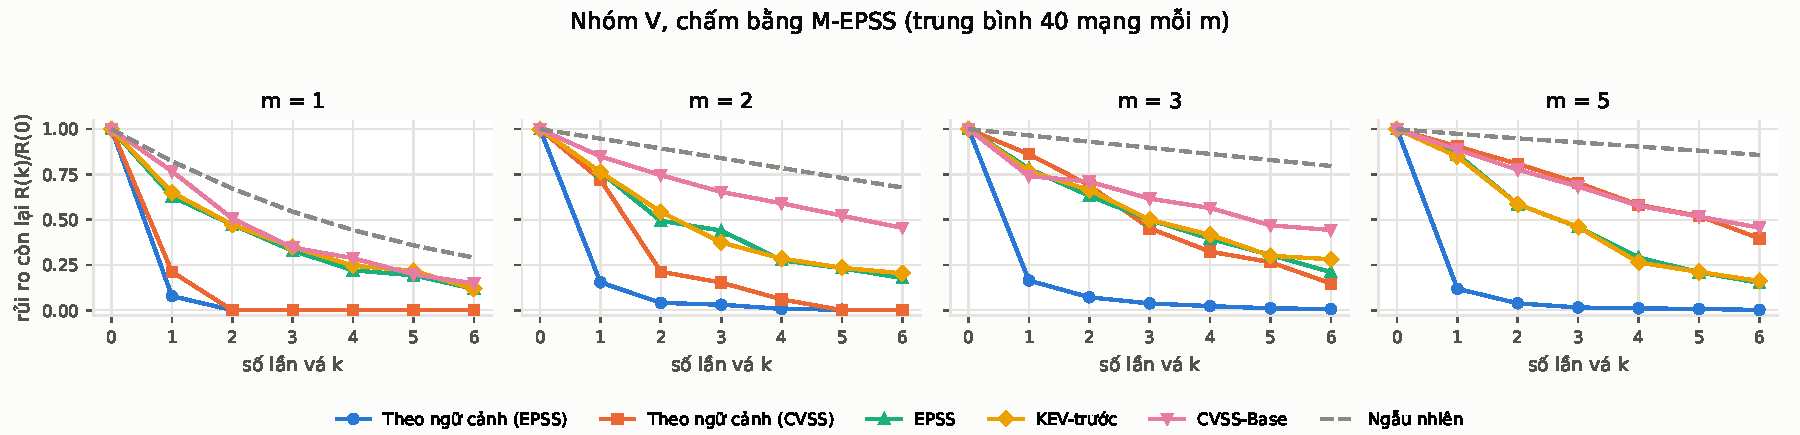
\includegraphics[width=\textwidth]{figures/V_Rk_epss.pdf}
\caption{Rủi ro còn lại $R(k)/R(0)$ theo số lần vá, chấm bằng M-EPSS.}
\end{figure}

\textbf{Phát hiện chính.}
\begin{enumerate}
  \item \textbf{Xét ngữ cảnh đường tấn công thắng rõ.} Chính sách theo ngữ cảnh thắng chính sách điểm dùng cùng nguồn dữ liệu ở 30--40/40 mạng, ở mọi $m$ và dưới cả ba mô hình chấm ($p \le 2\cdot 10^{-6}$). Ở $m = 1$ nó gần tối ưu (0,096 so với 0,095). Ví dụ cụ thể: EPSS và CVSS-Base vá trước CVE-2024-3094 (backdoor xz-utils, điểm 10, EPSS 0,91), nhưng máy đó không nằm trên đường tới tài sản nhạy cảm nên rủi ro không đổi.
  \item \textbf{Trong các thang điểm,} EPSS $\approx$ KEV-trước, tốt hơn CVSS-Base, tốt hơn ngẫu nhiên. Dưới M-CVSS, các chính sách điểm gần như vô dụng khi $m \ge 2$, vì nhiều CVE có cùng điểm khai thác.
  \item \textbf{Ngữ cảnh chỉ có lợi khi ước lượng xác suất đúng.} Xét đường tấn công nhưng dùng xác suất CVSS, khi chấm bằng M-EPSS ở $m = 5$, lại thua chính sách EPSS đơn giản: EPSS tốt hơn ở 28/40 mạng, $p = 0{,}002$. Vì vậy giả thuyết ``thứ hạng bền khi đổi mô hình'' chỉ đúng một phần.
\end{enumerate}

\textbf{Phân tích độ nhạy.} Có năm biến thể, công bố trước:
\begin{itemize}
  \item $K = 15$;
  \item 50\% CVE thuộc KEV;
  \item đội máy đồng nhất;
  \item $p_{\text{kev}} = 0{,}5$ và $p_{\text{kev}} = 0{,}99$.
\end{itemize}
Kết luận 1 giữ nguyên ở mọi biến thể ($p \le 6\cdot 10^{-6}$), và giá trị $p_{\text{kev}}$ gần như không ảnh hưởng. Hai kết quả có điều kiện:
\begin{itemize}
  \item ưu thế của EPSS so với CVSS-Base mất khi 50\% CVE thuộc KEV;
  \item nguy cơ khi xét ngữ cảnh mà dùng sai mô hình xác suất yếu đi, không còn ý nghĩa thống kê, ở các biến thể 50\% KEV và đội máy đồng nhất.
\end{itemize}

\section{So sánh hai giai đoạn và việc còn lại}

\begin{center}
\begin{tabular}{@{}Y{3cm}Y{5.8cm}Y{6.2cm}@{}}
\toprule
& AAPEF (giai đoạn 1) & AAPEF v2 (giai đoạn 2) \\
\midrule
Góc nhìn & Kẻ tấn công: tìm đường & Người phòng thủ: chọn lỗ hổng để vá \\
Câu hỏi & Thuật toán nào tối ưu, tốn bao nhiêu công & Chính sách vá nào giảm rủi ro nhiều nhất \\
Dữ liệu & Kịch bản tự thiết kế, vector CVSS & Snapshot NVD/KEV/EPSS có hash; mạng NASim \\
Đánh giá & Benchmark 27 kịch bản & 160 mạng, ba mô hình, Wilcoxon, độ nhạy \\
Vai trò của lõi & Là đối tượng nghiên cứu & Là thước đo rủi ro (dùng lại nguyên vẹn) \\
\bottomrule
\end{tabular}
\end{center}

\textbf{Hạn chế.} Kết quả chỉ đúng trong mô hình, với các giả định sau:
\begin{itemize}
  \item các bước tấn công độc lập;
  \item kẻ tấn công tối ưu và biết toàn bộ mạng;
  \item vá hoàn hảo và tức thời;
  \item chưa tính giá trị tài sản;
  \item CVE gắn theo vai trò, không theo đúng sản phẩm;
  \item mạng nhỏ (tối đa 18 máy).
\end{itemize}

\textbf{Hiện trạng và việc còn lại.} Phần kỹ thuật đã xong. Còn lại:
\begin{itemize}
  \item snapshot dữ liệu thứ hai (khoảng 10/11/2026) để kiểm tra độ ổn định theo thời gian;
  \item viết quyển đồ án;
  \item chuẩn bị slide bảo vệ.
\end{itemize}

\end{document}
